\section{Durchführung}
\label{sec:Durchfuehrung}

\subsection{Schallgeschwindigkeit und Dämpfung mit dem Impuls-Echo-Verfahren}
\label{sec:impEcho}

Es wird an insgesamt 7 Acrylzylindern nacheinander gemessen.
Zuert wird die Dicke des Zylinders mit einer Schieblehre bestimmt.
Dann wird der Zylinder auf ein Papiertuch gestellt und mit bidestilliertem Wasser mit einer 2MHz-Sonde gekoppelt.
Mit dem Impuls-Echo-Verfahren wird ein A-Scan durchgeführt und für den ersten und zweiten reflektierten Puls die Laufzeit, sowie Amplitude bestimmt.
Es wird mit dem größten Zylinder begonnen und die Amplitude des zweiten Pulses durch den Verstärker auf einen Wert zwischen 1 und 1,2 V geregelt.
Danach bleibt die Verstärkung für alle weiteren Messungen gleich eingestellt.
Aus den gemessenen Zeitunterschieden und den Zylinderlängen wird später in einem Plot mit Fit die Schallgeschwindigkeit aus der Steigung ermittelt.
Aus den Daten der Amplituden des zweiten Pulses kann dann die Dämpfung mit der Formel \ref{eqn:gl3} berechnet werden.

\subsection{Schallgeschwindigkeit mit dem Durchschallungs-Verfahren}
\label{sec:DurchSchall}

Es werden die selben Zylinder wie in Abschnitt \ref{sec:impEcho} verwendet.
Diese werden horizontal in eine schwarze Halterung gelegt und mit einem Koppelgel werden an beiden Stirnseiten die Sinden gekoppelt.
Im A-Scan wird die Laufzeit, die der Schallimpuls zum Durchlaufen des Zylinders benötigt, ausgemessen und erneut die Schallgeschwindigkeit berechnet.
Diese Ergebnisse werden mit den Ergebnissen aus Abschnitt \ref{sec:impEcho} verglichen.

\subsection{Spektrale Analyse und Cepstrum}
\label{sec:spectral}

Es werden zwei verschieden dicke Acrylplatten miteinander gekoppelt und oben drauf noch ein Acrylzylinder der Länge 4cm gekoppelt.
Dann werden im Impuls-Echo-Verfahren Mehrfachimpulse aufgenommen.
Der Acrylzylinder dient als Vorlaufstrecke, so dass die Mehrfachechos besser von dem Initialecho getrennt werden können.
Um zu beginnen wird die 2 MHz Sonde an den Zylinder gekoppelt.
Jetzt sind alle Gegenstände mit bidestilliertem Wasser gekoppelt.
Die Verstärkung wird so eingestellt, dass drei Mehrfachreflexionen zu sehen sind.
Mit diesen drei Reflexionen wird mit Hilfe der FFT-Funktion ein Spektrum und das Cepstrum der Sonde erzeugt.
Es soll die Laufzeit der drei Refelxionen gemessen werden und mit Hilfe der bestimmten Schallgeschwindigkeit wird die Dicke der Platten berechnet.
Genau so soll die Dicke mit den Peaks aus dem Cepstrum berechnet werden und das FFT-Spektrum interpretiert werden.

\subsection{Biometrische Untersuchung eines Augenmodells}
\label{sec:auge}

\begin{figure}
    \centering
    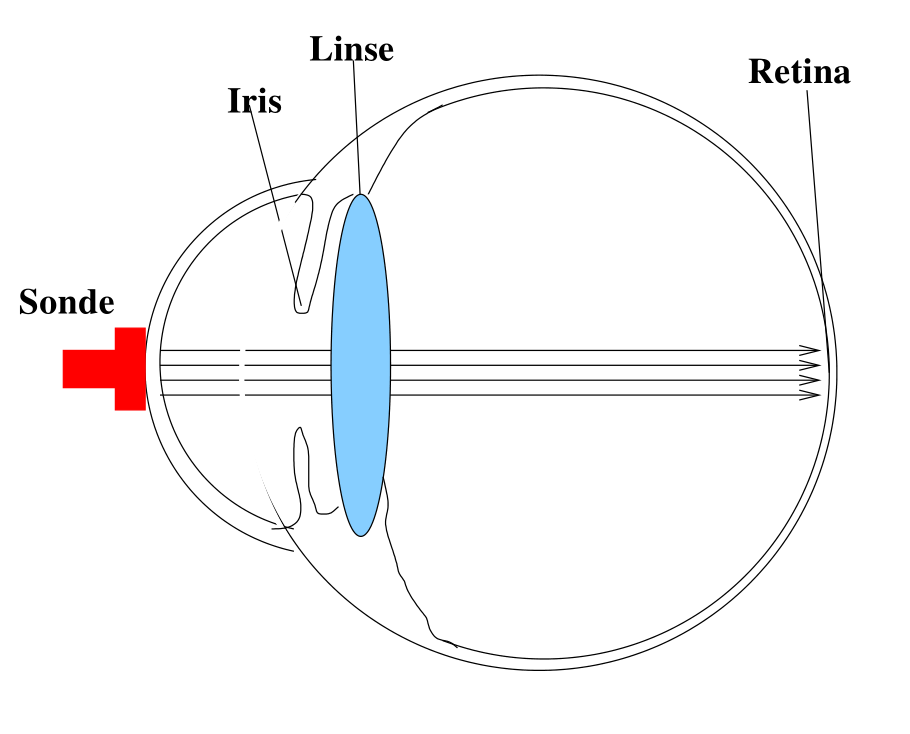
\includegraphics[width=6cm]{data/abb1.png}
    \caption{Augenmodell. \cite{US1}}
    \label{fig:modell}
  \end{figure}
  \FloatBarrier

Anhand eines Augenmodells (siehe Abb. \ref{fig:modell}) sollen die Abstände im Auge bestimmt werden.
Es sollen die Abmessungen des Auges mit dem Impuls-Echo-Verfahren ermittelt werden.
Die 2 MHz Sonde wird mit Koppelgel vorsichtig über die Hornhaut bewegt, bis ein Echo an der Rückwand der Retina zu sehen ist.
Mit einem A-Scan werden die Echos an den Grenzflächen der Iris, dem Linsenein- und ausgang und der Retina aufgenommen.
Danach werden aus der Laufzeit die Abmessungen des Auges bestimmt.
Es sind die unterschiedlichen Schallgeschwindigkeiten in der Linse $c_L = \SI{2500}{\meter\per\second}$ und in der Glaskörperflüssigkeit $c_{GK} = \SI{1410}{\meter\per\second}$ zu beachten.
